% This is a thesis template that attempts to conform to the guidelines
% published by UTRGV's Graduate School office.

% Please report any issues to
% https://github.com/UTRGV-SMSS/Thesis-Template/issues

% The author of this template is Guillermo Garza.


% Switch this line to the final option when submitting your thesis.
% This will correct counts and remove labels that are shown during draft mode
\documentclass[masters,draft]{UTRGVthesis}
%\documentclass[phd,draft]{UTRGVthesis}
%\documentclass[masters,final]{UTRGVthesis}
%\documentclass[masters,final, nodedication, noacknowledgments]{UTRGVthesis}


% Load your packages below.
% Make hyperref and showkeys come at the end of your loaded packages
% to make sure they are not over-written.  They redefine many
% standard LaTeX commands
\usepackage{docmute} % for inputting complete documents. Useful for LyX users
\usepackage{booktabs} % for better tables
\usepackage{microtype} % for better typography
\usepackage[colorlinks=false]{hyperref}  % for urls
%\usepackage{showkeys} % shows labels during draft mode
%\usepackage[document]{ragged2e} % uncomment for non-justified text
\usepackage{comment}
\usepackage{amsmath}

\usepackage{xcolor}   % added to show colors



% Uncomment the line below to check if text is aligned to margins
%\margins

% To change body font from Times Roman to Times New Roman, compile with XeLaTeX
% This assumes you have Times New Roman font installed in your machine
% WARNING! This will NOT change the font in Math Environments
\usepackage{ifxetex}
\ifxetex
   \usepackage{fontspec}
   \setmainfont{Times New Roman}
\fi

% this sets the name of the bibliography
% add \vspace{1cm} here to adjust vertical spacing after bibliography title
\renewcommand{\bibname}{BIBLIOGRAPHY}


% Insert your name and major here in the format shown
\Author{Andr\'es Cu\'ellar Vega}
\AuthorLastFirst{Cu\'ellar Vega, Andr\'es}
\Major{Physics}


% Insert your graduation date here
\Month{Dec}
\Year{2021}


% Insert the title of your thesis here.
% If you have a long title, split it between multiple lines using the \\ command
% Also, use comment characters to avoid unwanted spaces in the Abstract page
\Title{Titles Should Not Exceed Six Inches on One Line\\
and Be In The Inverted Pyramid Format\\
When Additional Lines Are Needed}


% Insert your research advisor and his title here
\Advisor{Dr. Andreas Hanke}
\AdvisorTitle{Chair of Committee}


% Insert the members of your committee here
% You can also give MemberA a special title
\MemberA{Dr. Carl Friedrich Gauss}  %\MemberATitle{Co-Chair of Committee}
\MemberB{Dr. G. F. Bernhard Riemann}
\MemberC{}
\MemberD{}
\MemberE{}


% Insert the text of your abstract below.
% The bibliography style "citation" required by the manual is automatically
% generated.  Specify the "final" option in the \documentclass to update the
% counts to the correct values.
\Abstract{%
An abstract is a brief summary often used to help the reader quickly
ascertain the paper's purpose.
}


% You can dedicate your paper here.  This is optional.
\Dedication{%
Dedication should be simple, in good taste, and fit on one page.
}


% Acknowledge those who helped and supported you here. This is optional.
\Acknowledgments{%
Acknowledgements should be simple, in good taste, and fit on one page.
}


% Insert your biographical sketch here.
\BiographicalSketch{%
A brief biographical sketch of the student is required as part of each thesis.
}



\begin{document}

% This starts page counting in Roman numerals
\frontmatter


% This command makes the formal preliminary pages.
% You can comment it out during the drafting process if you want to save paper.
%\makepreliminarypages


% These insert a table of contents, list of tables, and list of figures
%\tableofcontents
%\listoftables
%\listoffigures


% This starts regular page counting in Arabic numerals
\mainmatter

% This starts double-spaced text.  Opposite command is \singlespacing
\doublespacing


% OK. Everything is set up. Insert your thesis below.
% It's a good idea to split your thesis up into different files and use
% the \input command
%\chapter{Introduction} %\label{ch:intro}

\section{Zero Point Energy and the Dynamical Casimir Effect}
\section{Superconducting circuits and SQUIDS}
\section{DCE in Superconducting Circuits}
\section{Kronig-Penney Model in Solid State Physics}
 %\cite{Garza:2011fk}

\begin{comment}
\begin{figure}
  \centering
  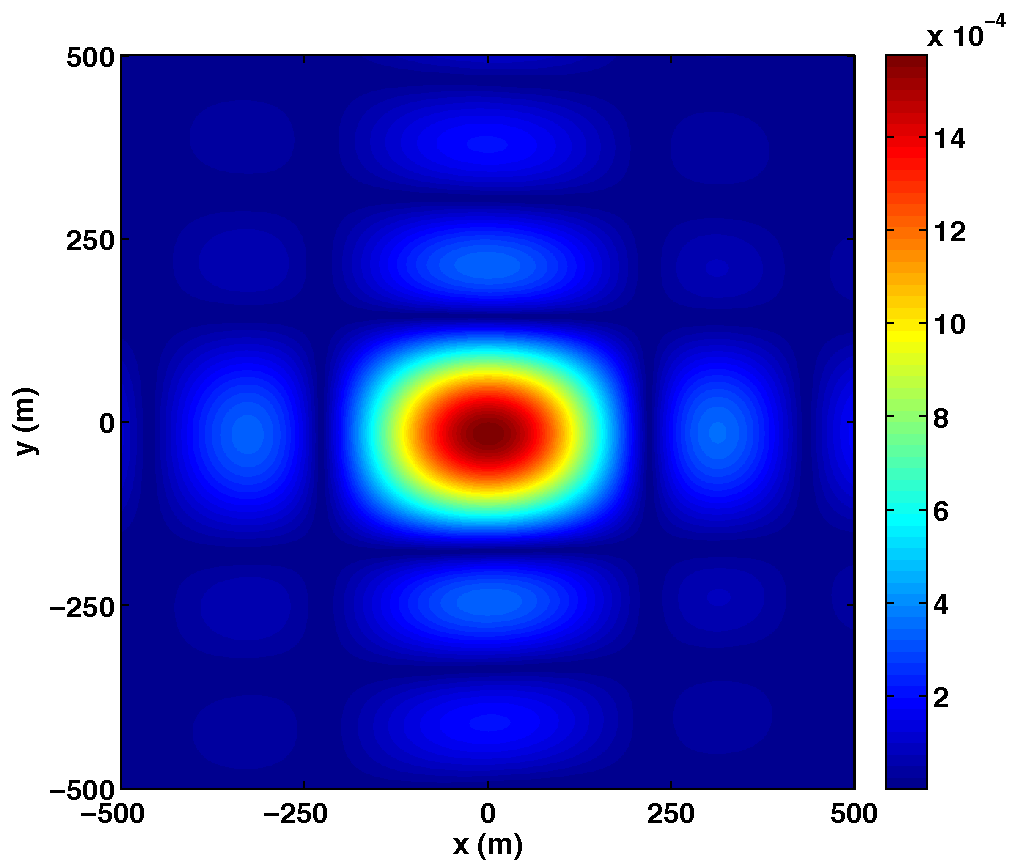
\includegraphics[scale=0.5]{figures/beamfootprint}
  \caption[Colorful Picture]{This is a colorful picture.}%
  \label{fig:flyover}
\end{figure}
\end{comment}


\begin{comment}
\begin{table}[p]
  \centering
\begin{tabular}{llr}
\toprule
\multicolumn{2}{c}{Item} \\
\cmidrule(r){1-2}
Animal    & Description & Price (\$) \\
\midrule
Gnat      & per gram    & 13.65      \\
          & each        & 0.01       \\
Gnu       & stuffed     & 92.50      \\
Emu       & stuffed     & 33.33      \\
Armadillo & frozen      & 8.99       \\
\bottomrule
\end{tabular}
  \caption[Table Example]{This table shows some data}%
  \label{tab:myfirsttable}
\end{table}
\end{comment}

%\chapter{Physical System}\label{ch:system}


\section{Dirac comb potential}

Testing laptop
x
\begin{equation} %\label{eq:einstein}
	V(x) = \delta(x-anx)
\end{equation}






\chapter{DCE in a Periodic Potential} %\label{ch:system}


\section{Circuit analysis for a 1D periodic potential quantum network}\label{sec:circ_an}
We want to study the DCE in a superconducting circuit as in (Johansson). We characterize the circuit in terms of dynamical fluxes $\Phi_i$. \color{blue} Assuming symmetric SQUIDs, the Lagrangian for this system is (cp. Johansson, Eq.\,(5))
\color{red} note edits. Use index $n$ for SQUIDs instead of $s$ \color{blue}
%
\begin{equation} \label{eq:lagn1}
\begin{split}
\mathcal{L} = \, & \frac{1}{2} \sum_i \left( \Delta x \, C_{0} \left(\dot{\Phi}_{i}\right)^{2} - 
\frac{\left(\Phi_{i+1}-\Phi_{i}\right)^{2}}{\Delta x \, L_{0}} \right)  \\[2mm]
& + \sum_n \left[ \frac{1}{2} \, C_{J,\,n} \left(\dot{\Phi}_{J,\,n} \right)^{2} \, + \, 
E_{J,\,n}(t) \cos\left(2\pi \frac{\Phi_{J,\,n}}{\Phi_0} \right) \right] \, \, .
\end{split}
\end{equation}
%
The terms on rhe r.h.s of the first line of Eq.\,(\ref{eq:lagn1}) describe sections of the CPW between the SQUIDs, where
$C_0, L_0$ are the characteristic capacitance and inductance per unit length of the CPW. 
The CPW is discretized in pieces $i$ of length $\Delta x$ with capacitance $\Delta x \, C_0$, 
inductance $\Delta x \, L_0$, and dynamical fluxes $\Phi_i$ \color{red}(see Figure X \{circuit diagram\})\color{blue}.   
The second line of Eq.\,(\ref{eq:lagn1}) describes the SQUIDs along the CPW indexed by $n$ 
with effective capacitance $C_{J,\,n}$ and flux $\Phi_{J,\,n}$ at node $n$. 
$\Phi_0 = h / (2 e)$ is the magnetic flux quantum.
The SQUIDs are separated by 
distance $\ell$ corresponding to the lattice constant of the 1D SQUID array. 
The Josephson energy $E_{J,\,n}(t)$ of SQUID $n$ is tunable
by the externally applied magnetic flux $\Phi_{\text{ext},\,n}(t)$ through the SQUID 
(cp. Johansson, Eq.\,(6)): 
%
\begin{equation} \label{eq:squidenergy}
    E_{J,\,n}(t) = 2 \, \epsilon_{J,\,n} 
    \left\vert \cos\left(\pi \frac{\Phi_{\text{ext},\,n}(t)}{\Phi_0}\right)\right\vert \, \, ,
\end{equation}
%
where $\epsilon_{J,\,n}$ is a constant energy parameter.

We assume that the plasma frequency $\omega_p$ of the SQUIDs far exceeds other characteristic frequencies 
in the circuit so that oscillations in the phase across the SQUIDs have small amplitude, i.e., 
$\Phi_{J,\,n} / \Phi_0 \ll 1$,
and the SQUIDs are operated in the phase regime where $E_{J,\,n} \gg (2e)^2 / (2C_{J,\,n})$. 
Using $\Phi_{J,\,n} / \Phi_0 \ll 1$ one may expand the cosine in Eq.\,(\ref{eq:lagn1}), 
resulting in a Lagrangian quadratic in $\Phi_{J,\,n}$ (dropping terms $E_{J,\,n}(t)$ 
independent of $\Phi_{J,\,n}$)
%
\begin{equation} \label{eq:lagn2}
\begin{split}
\mathcal{L} = \, & \frac{1}{2} \sum_i \left( \Delta x \, C_{0} \left(\dot{\Phi}_{i}\right)^{2} - 
\frac{\left(\Phi_{i+1}-\Phi_{i}\right)^{2}}{\Delta x \, L_{0}} \right)  \\[2mm]
& + \frac{1}{2} \sum_n \left( C_{J,\,n} \left(\dot{\Phi}_{J,\,n} \right)^{2} \, - \, 
 \left(\frac{2 \pi}{\Phi_0} \right)^2 E_{J,\,n}(t) \, \left( \Phi_{J,\,n} \right)^2 
\right) \, \, .
\end{split}
\end{equation}
%
From now on we assume that the intrinsic parameters of all SQUIDs are equal, i.e., 
$C_{J,\,n} = C_J$, $\epsilon_{J,\,n} = \epsilon_J$ for all $n$ in Eqs.\,(\ref{eq:lagn2}), (\ref{eq:squidenergy}).  
Moreover, we assume that the SQUID energy $E_{J,\,n}(t)$ in Eq.\,(\ref{eq:squidenergy}) 
can be expanded in a constant part plus weak harmonic drive 
(cp. Johansson, text page 6 bottom left)
%
\begin{equation} \label{eq:energyexp1}
E_{J,\,n}(t) = E_J^0 + \delta E_J \cos(\Omega_n \, t) 
\end{equation}
%
where $\delta E_J \ll E_J^0$ and $\Omega_n$ is the frequency of the external drive 
$\Phi_{\text{ext},\,n}(t)$ in Eq.\,(\ref{eq:squidenergy}).
As indicated in Eq.\,(\ref{eq:energyexp1}), we assume that the {\em static} part 
$E_J^0$ of $E_{J,\,n}(t)$ is the same for all SQUIDs. This assumption is crucial for our 
treatment of the {\em static} system (realized by a static applied magnetic flux $\Phi_{\text{ext}}$
for all SQUIDs) as a 1D periodic lattice with period $\ell$. However, the drive frequency 
$\Omega_n$ may be modulated along the 1D SQUID array, i.e., may differ for different SQUIDs $n$.   
This allows us to externally control the DCE radiation generated in the 1D SQUID array 
by different choices of the external drive frequency $\Omega_n$ as a function of $n$. 
However, in our intial treatment we will assume for simplicity that the drive frequency is the 
same for all SQUIDs, i.e., $\Omega_n = \Omega$ for all $n$, and use 
%
\begin{equation} \label{eq:energyexp2}
E_{J,\,n}(t) \equiv E_J(t) = E_J^0 + \delta E_J \cos(\Omega \, t) \qquad \text{for all} \, \, \, \, n \, \, . 
\end{equation}
%
With these assumptions, the Lagrangian takes the form
%
\begin{equation} \label{eq:lagn3}
\begin{split}
\mathcal{L} = \, & \frac{1}{2} \sum_i \left( \Delta x \, C_{0} \left(\dot{\Phi}_{i}\right)^{2} - 
\frac{\left(\Phi_{i+1}-\Phi_{i}\right)^{2}}{\Delta x \, L_{0}} \right)  \\[2mm]
& + \frac{1}{2} \sum_n \left( C_J \left(\dot{\Phi}_{J,\,n} \right)^{2} \, - \, 
 \left(\frac{2 \pi}{\Phi_0} \right)^2 E_J(t) \, \left( \Phi_{J,\,n} \right)^2 
\right) \, \, .
\end{split}
\end{equation}
%
with $E_J(t)$ from Eq.(\ref{eq:energyexp2}). 

\color{black}

If we assume the plasma frequency of the SQUIDs is far exceeding the characteristic frequencies of the circuit
$\Phi_J/\Phi_0 \ll 1$, and that SQUIDs are operated in the phase regime where $E_J \gg \frac{(2e)^2}{2C_J}$, we can write a quadratic Lagrangian, 
%
\begin{equation}
\mathcal{L}=\frac{1}{2}\sum_{i=1}^{\infty}\left(\Delta x C_{0} \left(\dot{\Phi}_{i}\right)^{2} - 
\frac{\left(\Phi_{i+1}-\Phi_{i}\right)^{2}}{\Delta x L_{0}}\right) %
 + \frac{1}{2} \sum_{n=1}^{N}\left(C_J\left(\dot{\Phi}_{J, n}\right)^{2}-\left(\frac{2\pi}{\Phi_{0}}\right)^{2} E_J(t) \, \left( \Phi_{J,\,n} \right)^2 \right).
\end{equation}
%
Following the canonical quantization procedure, we now find the Hamiltonian of the system by performing a Legendre transformation $\mathcal{H}=\sum_{i}\frac{\partial\mathcal{L}}{\partial\dot{\Phi}} \dot{\Phi} - \mathcal{L}$.
%
\begin{equation}
\mathcal{H}=\frac{1}{2}\sum_{i=1}^{\infty}\left[\frac{P_i^2}{\Delta x \, C_{0}} -\left(\frac{\left(\Phi_{i+1}-\Phi_{i}\right)^{2}}{\Delta x L_{0}}\right)\right] 
 + \frac{1}{2} \sum_{n=1}^{N}\left(\frac{P_n^2}{C_J}+\left(\frac{2\pi}{\Phi_{0}}\right)^{2} E_J(t) \, \left( \Phi_{J,\,n} \right)^2 \right).
\end{equation}
%
We obtain the dynamics of the system by using the Heisenberg equations of motion for $P_i$ and $P_s$. 
In the \color{blue} continuum limit
$(\Delta x \to 0)$, the flux field satisfies the 1-dimensional massless Klein-Gordon equation
%
\begin{equation}
\frac{\partial^2\Phi(x,t)}{\partial t^2} - v^2 \, \frac{\partial^2\Phi(x,t)}{\partial x^2} = 0
\end{equation}
%
\color{blue}
where $v = 1 / \sqrt{C_0 L_0}$ as the propagation speed in the CPW.
\color{black}

The Heisenberg equation for $P_n$ (in continuous limit) provides the boundary condition at the SQUID sites $x_n$.
\begin{equation}\label{eq:BC_field}
C_{J} \ddot{\Phi}_{n}+\hbar\left(\frac{2 \pi}{\Phi_{0}}\right)^{2} E_{j}(t) \Phi_{n} -\frac{\hbar}{L_{0}}\left(\left.\frac{\partial \Phi_{n}}{\partial x}\right|_{x_n^{+}}-\left.\frac{\partial \Phi_{n}}{\partial x}\right|_{x_n^{-}}\right)=0.
\end{equation}

\section{Periodic potential and Kronig-Penney model}\label{sec:Kronig-Penney}
%
\noindent
Let us first consider the background periodic potential in the static case where we apply a DC drive so that the SQUID energy $E_J(t) = E_J^0$ is constant. Following the canonical quantization procedure, 
\color{blue} we turn the classical flux field ${\Phi}_n(x,t)$ 
in compartment $n$ of the periodic array \color{red} (see Fig.\,X) \color{blue}
into a field operator $\hat{\Phi}_n(x,t)$, which is expanded in terms of 
annihilation and creation operators $\color{blue} \hat{a}_n(k)$ and 
$\color{blue} {\hat a}_n^\dagger(k)$:
%
\begin{equation} \label{eq:flux_field_orig}
    \hat{\Phi}_n(x,t) = \sqrt{\frac{\hbar}{2 C_0}} 
    \int_{-\infty}^{\infty}\frac{dk}{2 \pi} \frac{1}{\sqrt{\omega_k}}
    \left\{ \hat{a}_n(k) \psi_k(x)e^{-i \omega(k) \, t} + 
    \hat{a}_n^{\dagger}(k) \psi_k^*(x) e^{i \omega(k) \, t} \right\} \, \, .
\end{equation}
%
The annihilation and creation operators obey the commutation relations
%
\begin{equation} \label{eq:cra_orig}
    \left[ \hat{a}_n(k),{\hat a}_{n'}^\dagger(k') \right] = \delta_{nn'} \, 2 \pi \delta(k - k')
\end{equation}
%
and thus have units of $\text{length}^{1/2}$.
Equation (\ref{eq:flux_field_orig}) also incorporates the Bloch-type functions 
%
\begin{equation} \label{eq:psi1}
\psi_k(x) = e^{i k x} u_k(x) \, \, ,   
\end{equation}
%
where $u_k(x)$ has period $\ell$, i.e., $u_k(x + \ell n) = u_k(x)$ for all integers $n$.
The Bloch functions $\psi_k(x)$ in Eq.\,(\ref{eq:psi1}) are unitless, orthogonal with respect to 
the 1D wave vector $k$, and normalized such that
%
\begin{equation} \label{eq:psi1_norm_orig}
\int_{-\infty}^{\infty} dx \, \psi^*_k(x) \psi_{k'}(x) = 2 \pi \, \delta(k - k') \, \, .
\end{equation}
%
The prefactor $\displaystyle{\sqrt{\frac{\hbar}{2 C_0}}}$ in Eq.\,(\ref{eq:flux_field_orig}) is chosen 
to obtain the canonical commutation relation 
%
\begin{equation} \label{eq:commrelphi}
\left[ \hat{\Phi}_n(x,t), \hat{P}_n(x',t) \right] = i \hbar \delta(x-x')
\end{equation}
%
where $\hat{P}_n(x,t) = C_0 \displaystyle{\frac{d}{dt}} \hat{\Phi}_n(x,t)$ is the 
canonical conjugate of $\hat{\Phi}_n(x,t)$ and $C_0$ is the characteristic capacitance of the CPW per unit length. 
%
We now rewrite Eq.\,(\ref{eq:flux_field_orig}) in terms of unitless variables 
by expressing lenghts in units of $\ell$ and times in units of $\ell/v$
as outlined in \color{red} Section X:  \color{blue}  
%
\begin{equation} \label{eq:flux_field}
    \hat{\phi}_n(x,t) = 
    \int_{-\infty}^{\infty}\frac{dk}{2 \pi} \frac{1}{\sqrt{\omega_k}}
    \left[ \hat{a}_n(k) \psi_k(x)e^{-i \omega(k) \, t} + 
    \hat{a}_n^{\dagger}(k) \psi_k^*(x) e^{i \omega(k) \, t} \right]
\end{equation}
%
with the unitless field operator in compartment $n$ of the periodic array
%
\begin{equation} \label{eq:ufo}
\hat{\phi}_n(x,t) := \sqrt{\frac{2 C_0 v}{\hbar}} \, \hat{\Phi}_n(x,t) \, \, .
\end{equation}
%
Unitless annihilation and creation operators are defined by $\hat{a}_n(k)/\sqrt{\ell}$ 
and ${\hat a}_{n}^\dagger(k) / \sqrt{\ell}$ and again denoted by
$\hat{a}_n(k)$, ${\hat a}_{n}^\dagger(k)$ to keep the notation simple. 
They obey the commutation relations 
%
\begin{equation} \label{eq:cra}
    \left[ \hat{a}_n(k),{\hat a}_{n'}^\dagger(k') \right] = \delta_{nn'} \, 2 \pi \delta(k - k') \, \, .
\end{equation}
%
All variables in Eq.\,(\ref{eq:flux_field}) are unitless by expressing lengths in units of $\ell$
and times in units of $\ell/v$.
%
\color{black}
%
%
Given the time dependence of the flux field $\hat{\phi}_n(x,t)$, we can write our boundary condition (\ref{eq:BC_field}) as
%
\begin{equation}
\left[-\omega^2 C_{J}+\hbar\left(\frac{2 \pi}{\Phi_{0}}\right)^{2} E_{j}^0\right]\hat{\phi}_n(x,t) -\frac{\hbar}{L_{0}}\left(\left.\frac{\partial \hat{\phi}_n(x,t)}{\partial x}\right|_{x_n^{+}}-\left.\frac{\partial \hat{\phi}_n(x,t)}{\partial x}\right|_{x_n^{-}}\right)=0.
\end{equation}
%
By construction, we require the Bloch functions $\psi_k(x)$ to be eigenfunctions of
%
\begin{equation}\label{eq:bloch_eigenvalproblem}
\left.\frac{\partial\psi_{k}(x)}{\partial x}\right|_{x_n^{+}}-\left.\frac{\partial\psi_{k}(x)}{\partial x}\right|_{x_n^{-}}=\lambda \psi_k(x),
\end{equation}
%
where $\lambda$ is defined as:
%
\begin{equation}
\lambda = \left(\frac{L_0}{\hbar}\right)  
\left[-\omega^2 C_{J}+\hbar\left(\frac{2 \pi}{\Phi_{0}}\right)^{2} E_{j}^0\right]
\end{equation}
%
as well as to satisfy the continuity condition
%
\begin{equation}\label{eq:continuity_bloch}
\biggl.\psi_{k}(x)\biggl|_{x=x_{n}}=\biggl.\psi_{k}(x)\biggr|_{x=x_{n}^{+}}.
\end{equation}
%
We express solutions as
%
\begin{align}
\psi_{k,n}(x) = A_n e^{i\omega(x}-n) + B_n e^{-i\omega(x-n)},\hspace{16ex} n-1 < x < n,\\
\psi_{k,n+1}(x) = A_{n+1} e^{i\omega(x-n-1)} + B_{n+1} e^{-i\omega(x-n-1)}, \hspace{10ex} n < x < n+1.
\end{align}
%
We follow a standard procedure to find wavefunction solutions to the Kronig Penney model, employing a transfer matrix method to find solutions for $A_{n+1}, B_{n+1}$ in terms of $A_n, B_n$. Using (\ref{eq:continuity_bloch}), we can express (\ref{eq:bloch_eigenvalproblem}), with a transfer matrix
%
\begin{equation}
 \begin{pmatrix}
 A_{n+1} \\ B_{n+1}
 \end{pmatrix}
 = T 
 \begin{pmatrix}
 A_n \\ B_n
 \end{pmatrix}
\end{equation}{}
%
We construct matrix $T=PL^{-1}VL$ by defining the following matrices 
%
\begin{align}
L = \begin{pmatrix}
1 & 1 \\
i\omega & -i\omega
\end{pmatrix} \\
%
V = \begin{pmatrix}
1 & 0 \\
\lambda & 1
\end{pmatrix} \\
%
P = \begin{pmatrix}
e^{i\omega} & 0 \\
0 & e^{-i\omega}.
\end{pmatrix}
\end{align} 
%
We then find eigenvalues for $T$
\begin{equation}
    \mu_{(1/2)} = \cos{\omega} + \frac{\lambda}{2\omega}\sin{\omega}\mp i \sqrt{1-\left(\cos{\omega} + \frac{\lambda}{2\omega}\sin{\omega}}\right)^2}
\end{equation}
%
The determinant of $T$ is 1 (det $T = 1$), thus the eigenvalues of this matrix fulfill $\mu_1 \cdot \mu_2 = 1$. We find that $|\mu_1| = |\mu_2|=1$, and thus we can define $\tilde{k}$ as $e^{\pm ik} = \mu_{(1/2)}$.\\
We find a band structure with $k$-bands determined by the dispersion relation
\begin{equation}
    \cos{k} = \cos{\omega} + \frac{\lambda}{2\omega}\sin{\omega}
\end{equation}
%
where physical states correspond to solutions such that
\begin{equation}\label{eq:band_condition}
    \left|\cos\omega} + \frac{\lambda}{2\omega}\sin{\omega}\right|\leq 1.
\end{equation}
%
The (normalized) eigenvectors of $T$ are given by:
\begin{gather}
    \hat{V}^{(1)}
    = N
    \begin{pmatrix}
    e^{i\omega}\left\lbrace-\cos{\omega} + \frac{\lambda}{2\omega}\sin{\omega} - \frac{2\omega}{\lambda}\sqrt{1-\left(\cos{\omega+\frac{\lambda}{2\omega}\sin{\omega}}\right)^2}
    \right\rbrace \\ 1 \end{pmatrix} \\
    \hat{V}^{(2)}
    = N
    \begin{pmatrix}
    \left\lbrace-\cos{\omega} + \frac{\lambda}{2\omega}\sin{\omega} + \frac{2\omega}{\lambda}\sqrt{1-\left(\cos{\omega+\frac{\lambda}{2\omega}\sin{\omega}}\right)^2}
    \right\rbrace \\ e^{-i\omega} \end{pmatrix}
\end{gather}
%
where $N$ is a normalization constant. From these eigenvectors, we can obtain the states of the system at the $n$th lattice site by plugging in a state $\psi_{k,n=0}(x)$ and using the eigenvalue equation for the transfer matrix $T$.
\begin{equation}
    \begin{pmatrix}
    A_n^{(1/2)} \\ B_n^{(1/2)}
    \end{pmatrix}
    = e^{\pm i\tilde{k}n} 
    \begin{pmatrix}
    A_0^{(1/2)} \\ B_0^{(1/2)}
    \end{pmatrix}
\end{equation}
%
Thus, we arrive at functions $\psi_{k}(x)$, which we can write in the Bloch form
\begin{equation}\label{eq:bloch_waves}
    \psi_{k}^R (x) =e^{ikx} \hat{u}_{k}^{(1)}(\tilde{x}), \hspace{12pt}  \psi_{k}^L(x) =e^{-ikx} \hat{u}_{k}^{(2)}(x) 
\end{equation}
%
Where $\hat{u}_{k}^{(1/2)}$ are the normalized forms of periodically repeated functions
\begin{gather}
      u_{k}^{(1)}(x) = 
      \frac{A_0^{(1)} e^{i(\omega-k)(x-1)} + B_0^{(1)} e^{-i(\omega+k)(x-1)}}{A_0^{(1)}+B_0^{(1)}}\\
       u_{k}^{(2)}(x) =
      \frac{A_0^{(2)} e^{i(\omega+k)(x-1)} + B_0^{(2)} e^{-i(\omega-k)(x-1)}}{A_0^{(2)}+B_0^{(2)}}
\end{gather}
%
normalized such that
\begin{equation}
\int_0^1 \hat{u}_{k} (\hat{u}_{k})^* dx = 1
\end{equation}
%
Since the functions \ref{eq:bloch_waves} form a complete set, we can use them to expand our flux field as in \ref{eq:flux_field}.
%
\section{Static Flux Solution}\label{eq:Static_Flux}

We proceed to obtain solutions for the problem with applied static magnetic flux. Taking the Fourier transform of the field \ref{eq:flux_field}, expanded in terms of the bloch waves
\begin{equation}
    \Phi(x, \mu = \int_{-\infty}^\infty \Phi(x,t) e^{i\mu t} dt
\end{equation}

We obtain the following forms for the field:
\begin{gather}
    \Phi(x,\mu) = \sqrt{\frac{\hbar}{2 C_0}} \left| \left.\frac{d\omega}{dk}\right|_{\omega=\mu}\right|^{-1}\frac{1}{\sqrt{\mu}}\biggl\lbrace a_R(K) \psi^R_K(x) + a_L(K)\psi_K^L(x)\biggr\rbrace, \hspace{12pt} \mu > 0.\\
    \Phi(x,\mu) = \sqrt{\frac{\hbar}{2 C_0}} \left| \left.\frac{d\omega}{dk}\right|_{\omega=\mu}\right|^{-1}\frac{1}{\sqrt{|\mu|}}\biggl\lbrace a_R^\dagger(K) \left[\psi^R_K(x)\right]^* + a_L^\dagger(K)\left[\psi_K^L(x)\right]^*\biggr\rbrace, \hspace{12pt} \mu < 0.
\end{gather}

Where we have used (\ref{eq:bloch_waves}), defining $K = |k|$. As well as 
\begin{equation}
    a(K) = 
    \begin{cases}
    a_R(K) &\text{if k > 0,}\\
    a_L(K) &\text{if k < 0.}
    \end{cases}
\end{equation}




Which we input into the  boundary condition \ref{eq:BC_field} to obtain

\begin{equation}
    \left[a_R(K) - b_R(K)\right]\mathcal{A}_K + \left[a_L(K) - b_L(K)\right]\mathcal{A}_K^* = 0 
\end{equation}

where we define
\begin{gather}
    \mathcal{C}_K = \left.u_K(x)\right|_{x=x_s}\\
    \mathcal{D}_K = \left.u_K^{\prime}(x)\right|_{x=x_s}\\
    \mathcal{A}_K = ik\mathcal{C}_K + \mathcal{D}_K
\end{gather}


% This makes the bibliography.
% Enter your references in the BibTex file "references.bib"
% You can find bibtex info from Google Scholar.
\bibliographystyle{siam}
\bibliography{references}


% Uncomment the \appendix macro below for appendices
% Insert appendix chapters after the macro
%\appendix


% This inserts your Biographical Sketch
%\biographypage

\end{document}
